% !TEX root = ../main.tex

\section{Results}
To test the perceptron compiling and training, 5 different truth tables were used, ranging from 2 to 3 inputs. The correct output was reached after 16-23 iterations of the learning algorithm. Input sizes greater than 3 was not tested, as the training time increases exponentially in time with the input size.

\subsection{2-input AND}

\begin{figure}[H]
  \begin{subfigure}[t]{.49\columnwidth}

      \centering
    \begin{tabular}[b]{ccc}
      \hline
      \multicolumn{1}{l}{\textbf{Input 1}} & \multicolumn{1}{l}{\textbf{Input 2}} & \multicolumn{1}{l}{\textbf{Output}} \\
      \hline
      0                                    & 0                                    & 0                                   \\
      0                                    & 1                                    & 0                                   \\
      1                                    & 0                                    & 0                                   \\
      1                                    & 1                                    & 1 \\
      \hline
    \end{tabular}
    \caption{Truth table for the 2-input AND gate.}
    \label{and_table}
  \end{subfigure}
  \begin{subfigure}[t]{.49\textwidth}
    \includegraphics[width=\textwidth]{figures/trained_2_and.tikz}
    \caption{Diagram of the 2-input AND with correct weights and threshold.}
  \end{subfigure}
\hfill
\begin{subfigure}[t]{\textwidth}
  \centering
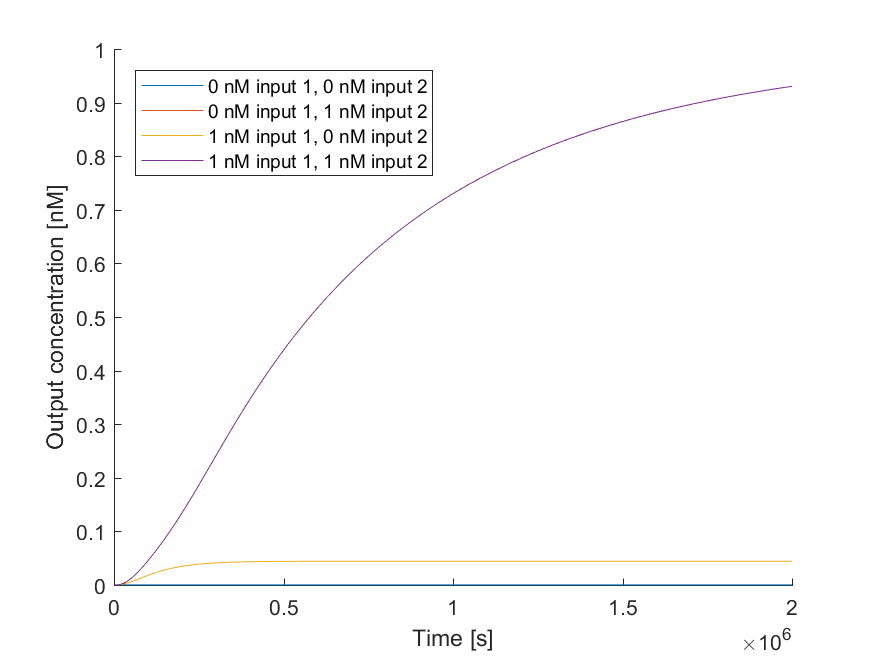
\includegraphics[width=\textwidth]{images/and_simulation.png}
\caption{Time analysis of the 2-input AND.}
\label{}
\end{subfigure}
\caption{Simulation results of the trained 2-input AND gate. The network is trained to activate when both of the inputs are active. The correct output was obtained after 21 iterations of the training algorithm, with a weight of 1.9 for all inputs, and a threshold of 10.}
\end{figure}

\subsection{2-input OR}

\begin{figure}[H]
  \begin{subfigure}[t]{.49\columnwidth}

      \centering
    \begin{tabular}[b]{ccc}
      \hline
    \multicolumn{1}{l}{\textbf{Input 1}} & \multicolumn{1}{l}{\textbf{Input 2}} & \multicolumn{1}{l}{\textbf{Output}} \\
    \hline
    0                                    & 0                                    & 0                                   \\
    0                                    & 1                                    & 1                                   \\
    1                                    & 0                                    & 1                                   \\
    1                                    & 1                                    & 1 \\
    \hline
    \end{tabular}
    \caption{Truth table for the 2-input OR gate.}
    \label{and_table}
\end{subfigure}
\begin{subfigure}[t]{.49\textwidth}
  \includegraphics[width=\textwidth]{figures/trained_2_or.tikz}
  \caption{Diagram of the 2-input OR with correct weights and threshold.}
\end{subfigure}
\hfill
\begin{subfigure}[t]{\textwidth}
  \centering
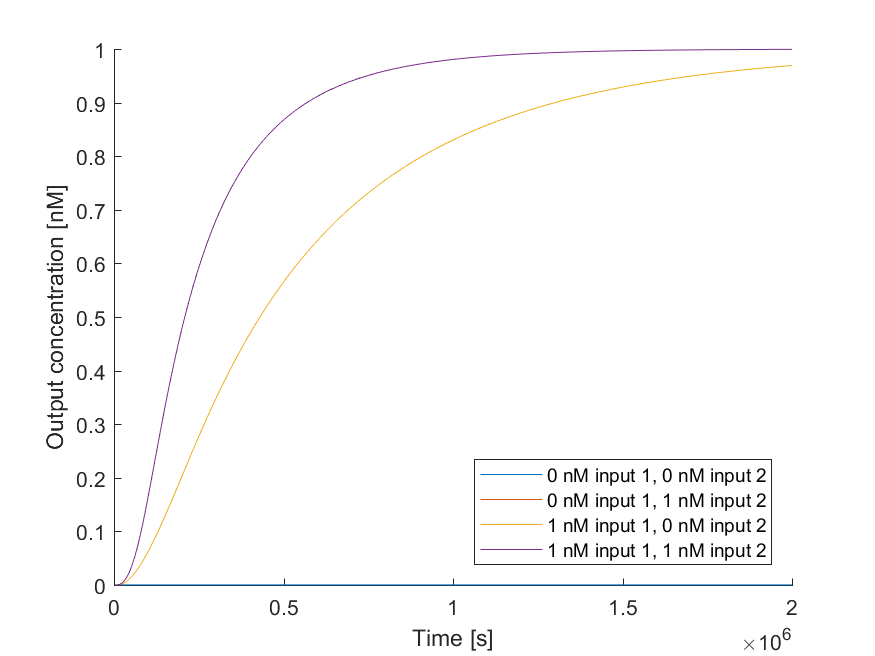
\includegraphics[width=\textwidth]{images/or_simulation.png}
\caption{Time analysis of the 2-input OR.}
\label{}
\end{subfigure}
\caption{Simulation results of the trained 2-input OR gate. The network is trained to activate when one of the inputs is active. The correct output was obtained after 22 iterations of the training algorithm, with a weight of 2.1 for all inputs, and a threshold of 10.}
\end{figure}

\subsection{3-input AND}

\begin{figure}[H]
  \begin{subfigure}[t]{.49\columnwidth}
    \begin{adjustbox}{width=\textwidth}
    \begin{tabular}[b]{cccc}
      \hline
    \multicolumn{1}{l}{\textbf{Input 1}} & \multicolumn{1}{l}{\textbf{Input 2}} & \multicolumn{1}{l}{\textbf{Input 3}} & \multicolumn{1}{l}{\textbf{Output}} \\
    \hline
    0 & 0                                    & 0                                    & 0                                   \\
    0 & 0                                    & 1                                    & 0                                   \\
    0 & 1                                    & 0                                    & 0                                   \\
    0 & 1                                    & 1                                    & 0                                   \\
    1 & 0                                    & 0                                    & 0                                   \\
    1 & 0                                    & 1                                    & 0                                   \\
    1 & 1                                    & 0                                    & 0                                   \\
    1 & 1                                    & 1                                    & 1                                   \\

    \hline
    \end{tabular}
  \end{adjustbox}
    \caption{Truth table for the 3-input AND gate.}
    \label{and_table}
\end{subfigure}
\begin{subfigure}[t]{.49\textwidth}
  \includegraphics[width=\textwidth]{figures/trained_3_and.tikz}
  \caption{Diagram of the 3-input AND with correct weights and threshold.}
\end{subfigure}
\hfill
\begin{subfigure}[t]{\textwidth}
  \centering
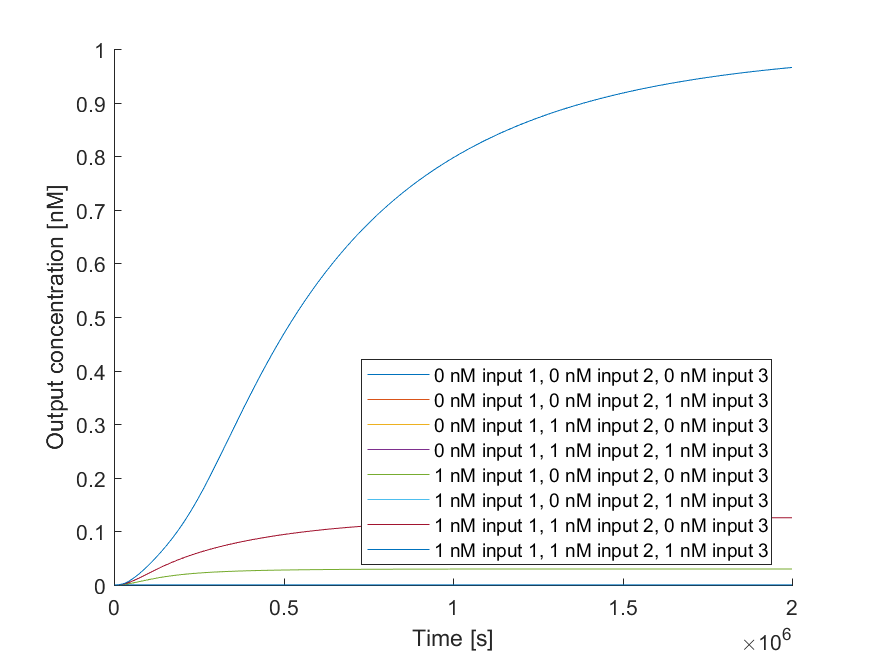
\includegraphics[width=\textwidth]{images/and_simulation_3input.png}
\caption{Time analysis of the 3-input AND.}
\label{}
\end{subfigure}
\caption{Simulation results of the trained 3-input AND gate. The network is trained to activate when all of the inputs are active. The correct output was obtained after 14 iterations of the training algorithm, with a weight of 1.2 for all inputs, and a threshold of 10.}
\end{figure}

\subsection{3-input 1-OR}

\begin{figure}[H]
  \begin{subfigure}[t]{.49\columnwidth}

      \begin{adjustbox}{width=\textwidth}
    \begin{tabular}[b]{cccc}
      \hline
    \multicolumn{1}{l}{\textbf{Input 1}} & \multicolumn{1}{l}{\textbf{Input 2}} & \multicolumn{1}{l}{\textbf{Input 3}} & \multicolumn{1}{l}{\textbf{Output}} \\
    \hline
    0 & 0                                    & 0                                    & 0                                   \\
    0 & 0                                    & 1                                    & 1                                   \\
    0 & 1                                    & 0                                    & 1                                   \\
    0 & 1                                    & 1                                    & 1                                   \\
    1 & 0                                    & 0                                    & 1                                   \\
    1 & 0                                    & 1                                    & 1                                   \\
    1 & 1                                    & 0                                    & 1                                   \\
    1 & 1                                    & 1                                    & 1                                   \\

    \hline
    \end{tabular}
  \end{adjustbox}
    \caption{Truth table for the 3-input 1-OR gate.}
    \label{and_table}
\end{subfigure}
\begin{subfigure}[t]{.49\textwidth}
  \includegraphics[width=\textwidth]{figures/trained_3_1_or.tikz}
  \caption{Diagram of the 3-input 1-OR with correct weights and threshold.}
\end{subfigure}
\hfill
\begin{subfigure}[t]{\textwidth}
  \centering
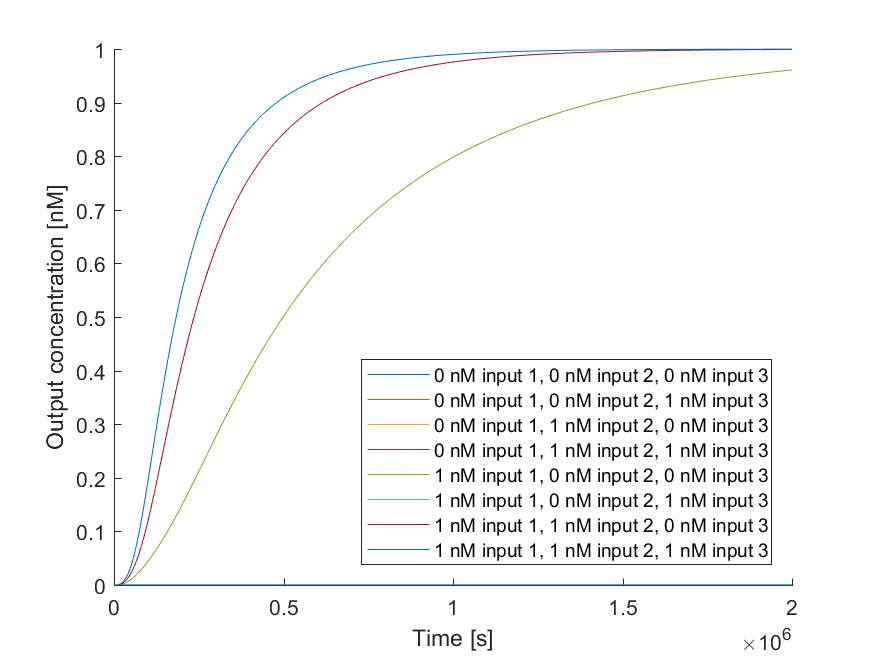
\includegraphics[width=\textwidth]{images/or_1_simulation_3input.png}
\caption{Time analysis of the 3-input 1-OR.}
\label{}
\end{subfigure}
\caption{Simulation results of the trained 3-input 1-OR gate. The network is trained to activate when at least 1 of the inputs is active. The correct output was obtained after 16 iterations of the training algorithm, with a weight of 1.3 for all inputs, and a threshold of 10.}
\end{figure}

\subsection{3-input 2-OR}


\begin{figure}[H]
  \begin{subfigure}[t]{.49\columnwidth}
    \begin{adjustbox}{width=\textwidth}
    \begin{tabular}[b]{cccc}
      \hline
    \multicolumn{1}{l}{\textbf{Input 1}} & \multicolumn{1}{l}{\textbf{Input 2}} & \multicolumn{1}{l}{\textbf{Input 3}} & \multicolumn{1}{l}{\textbf{Output}} \\
    \hline
    0 & 0                                    & 0                                    & 0                                   \\
    0 & 0                                    & 1                                    & 0                                   \\
    0 & 1                                    & 0                                    & 0                                   \\
    0 & 1                                    & 1                                    & 1                                   \\
    1 & 0                                    & 0                                    & 0                                   \\
    1 & 0                                    & 1                                    & 1                                   \\
    1 & 1                                    & 0                                    & 1                                   \\
    1 & 1                                    & 1                                    & 1                                   \\

    \hline
    \end{tabular}
  \end{adjustbox}
    \caption{Truth table for the 3-input 2-OR gate.}
    \label{and_table}
\end{subfigure}
\begin{subfigure}[t]{.49\textwidth}
  \includegraphics[width=\textwidth, valign=c]{figures/trained_3_2_or.tikz}
  \caption{Diagram of the 3-input 2-OR with correct weights and threshold.}
\end{subfigure}
\hfill
\begin{subfigure}[t]{\textwidth}
  \centering
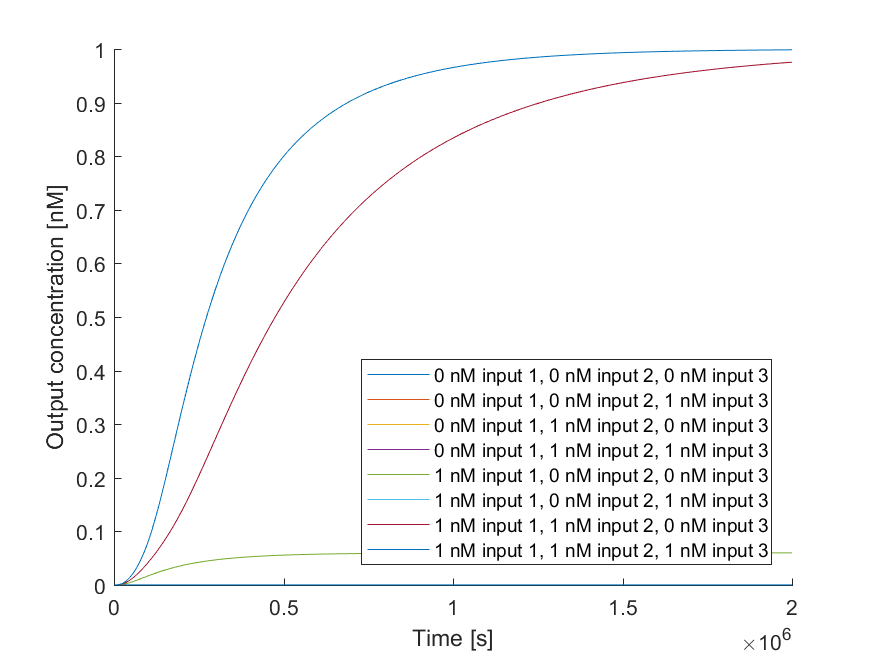
\includegraphics[width=\textwidth]{images/or_2_simulation_3input.png}
\caption{Time analysis of the 3-input 2-OR.}
\label{}
\end{subfigure}
\caption{Simulation results of the trained 3-input 2-OR gate. The network is trained to activate when at least 2 of the inputs is active. The correct output was obtained after 15 iterations of the training algorithm, with a weight of 1.4 for all inputs, and a threshold of 10.}
\end{figure}
